\documentclass[]{article}
\usepackage{float}
\usepackage{multicol}
\usepackage[a4paper, margin=0.68in]{geometry}
\usepackage[siunitx]{circuitikz}
\usepackage{siunitx}
\usepackage{tikz}
\usetikzlibrary{shapes,arrows}
\usepackage{verbatim}
\usepackage{lscape}
\usepackage{listings}
\usepackage{courier}
\usepackage{gensymb}
\usepackage{amsmath,amsfonts,mathtools,amssymb}
%opening
\title{ECEN405 Assignment 1}
\author{Keshav Raj 300418412\\Lab Partner: Tim Loretto}

\begin{document}
\tikzstyle{block} = [draw, fill=blue!20, rectangle, 
minimum height=3em, minimum width=6em]
\tikzstyle{sum} = [draw, fill=blue!20, circle, node distance=1cm]
\tikzstyle{input} = [coordinate]
\tikzstyle{output} = [coordinate]
\tikzstyle{pinstyle} = [pin edge={to-,thin,black}]
\maketitle


\begin{multicols}{2}
	\section{Question 1}
	\subsection{a)}
	In order to ensure 80W can be delivered to a $4\Omega$ impedance load, a value for the full voltage swing range must be calculated which allows enough current to flow through the load to dissipate 80W through it. The voltage must be within 33V which is the maximum that one channel of the power supply can output and the current must be less than 6A which is the maximum two of the banks hooked in parallel can output.
	The following is the calculation of the required values:
	\begin{equation*}
	\begin{split}
	80&=IV\\
	80&=4I^2\\
	\frac{80}{V}&=I\\
	80&=4\left( \frac{80}{V} \right)^2\\
	80&=4\left( \frac{6400}{V^2} \right)\\
	80&=\frac{25600}{V^2}\\
	\frac{25600}{80}&=V^2\\
	V&=\sqrt{320}\\
	V&=17.888V\\
	I&=4.472A\\  
	\end{split}
	\end{equation*}
	\subsection{b)}
	In order to achieve the 10Hz to 200Hz bandwidth, firstly the triangle wave generator must be a high enough frequency to modulate the input signal without causing any aliasing. In order to ensure this, the triangle wave must be at least 10 times greater than the highest frequency component of the input signal. However, without filtering the input, we cannot be sure what the highest frequency component could be, therefore a bandpass filter at the input is required. The following constitutes the design for a cascaded sallen-key lowpass and high pass filter which are both chebyshev 3th order filters.
\end{multicols}
	\begin{figure}[H]
		\centering
		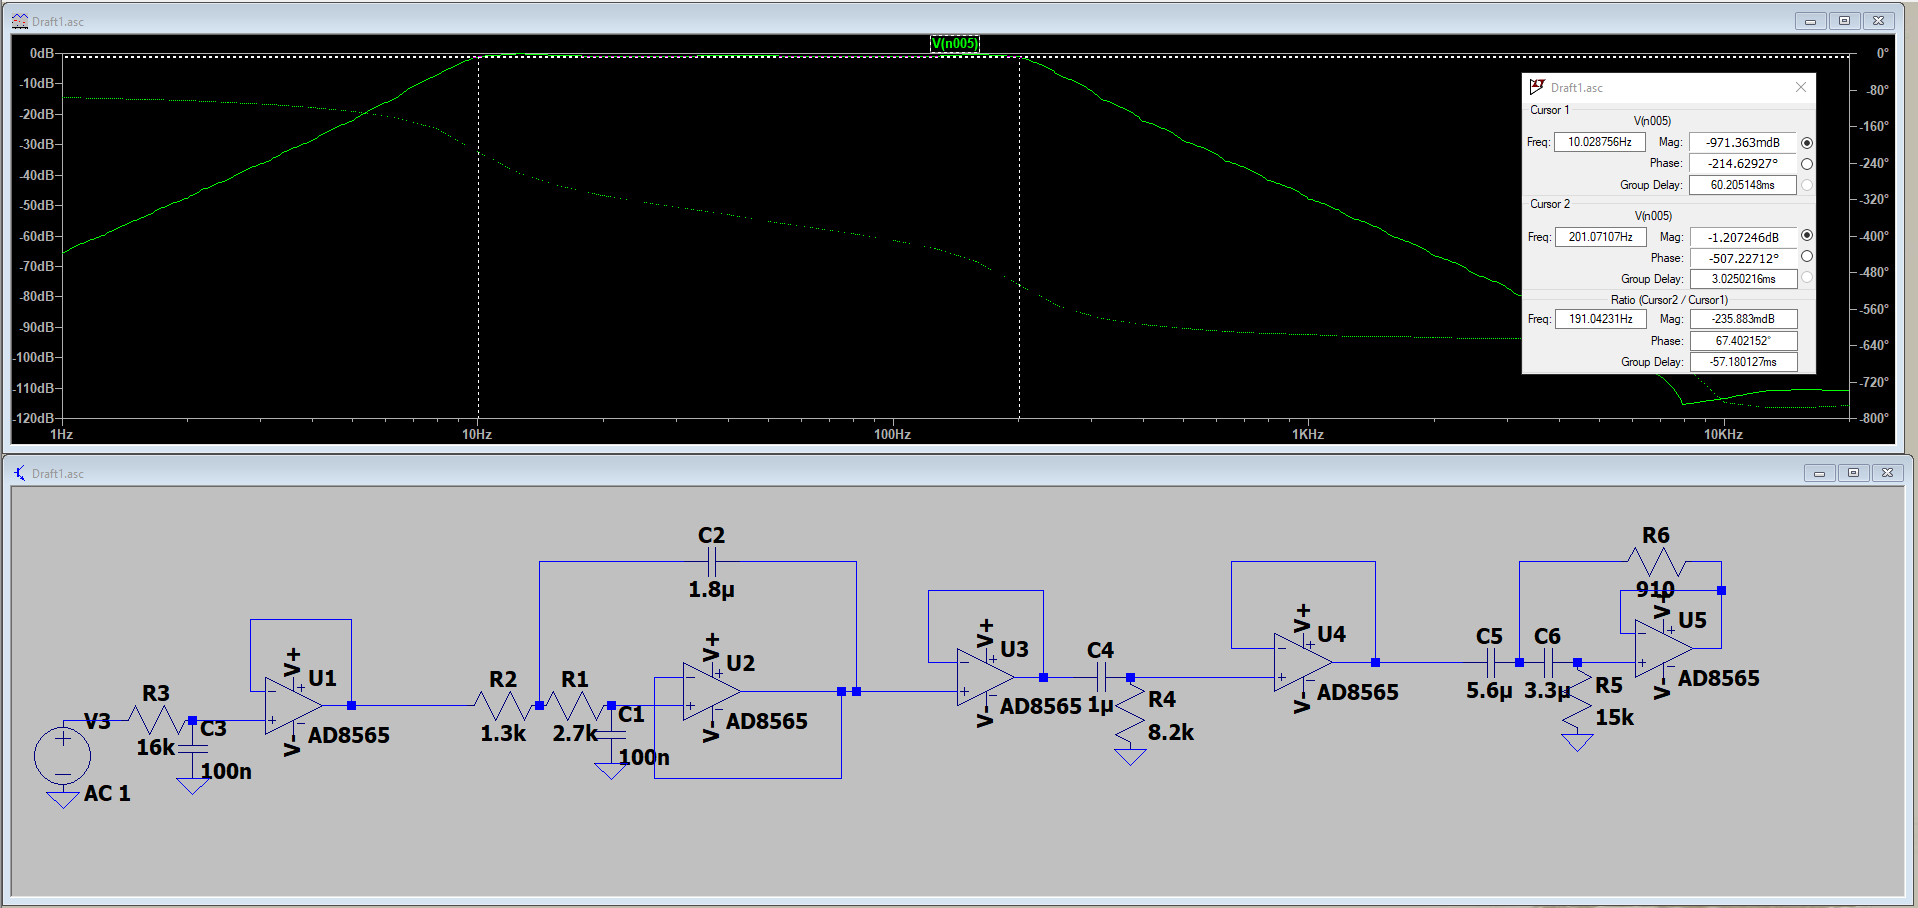
\includegraphics[width=1\linewidth]{screenshot001}
		\caption{Designed Filter simulated in LTSpice}
		\label{fig:screenshot001}
	\end{figure}
\begin{multicols}{2}
	This would mean that the triangle wave can now be at a frequency of 2000Hz or greater to ensure correct modulation of the input signal.
	\subsection{c)}
	In order to ensure that a signal of 1V amplitude (or 2Vpp) can be modulated, the input triangle wave to the comparator must have an amplitude of slightly over 2V to prevent output saturation. A value of 2.1V for the maximum amplitude of the triangle wave will suffice. If the triangle wave's amplitude is unable to be easily adjusted, the passband gain of the input filters can instead be adjusted to achieve the same required comparator level.
	The triangle wave from the oscillator will have a DC offset that will likely be around 1V. This can either be AC coupled which will distort the triangle wave (as it is not a pure sinusoid) or the input signal can be offset as well to the same level, this can either be done using a clamping circuit (not preferred), a simple voltage divider with a DC decoupling capacitor or a summing amplifier. It is preferred to use a summing amplifier as the clamping circuit is difficult to implement while the decoupling capacitor acts as an extra low pass filter which may alter the expected spectrum of the input signal.
	These additions will ensure that the input signal and the triangle wave can be compared to each other easily with the comparator and ensure a full swing of PWM duty cycle with minimal wave clipping on the output.\\
	As gate driver generally accept a 3.3V or 5V logic signal, this PWM output must be amplified to one of the logic standards, this can be done with a simple non-inverting amplifier.
\end{multicols}
	\section{Q2}
	The following diagram shows the selected design:
	\begin{figure}[H]
		\centering
		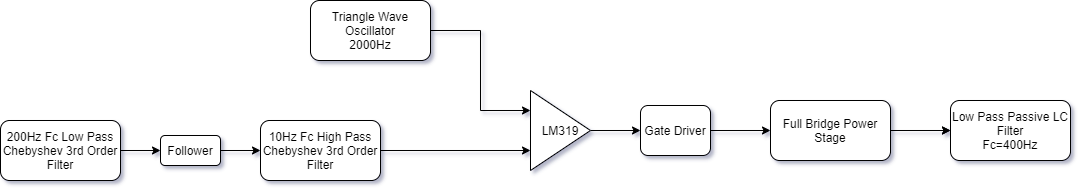
\includegraphics[width=1\linewidth]{Topology}
		\caption{D Class amplifier design}
		\label{fig:untitled-diagram-4}
	\end{figure}
\begin{multicols}{2}
	The first input low pass filter is a 3rd order chebyshev sallen-key topology filter. The output from this filter is cascaded with a voltage follower to a 10Hz high pass filter of the same type as the first low pass filter. The output from here can be offset if required to match the same offset of the triangle wave oscillator output.\\
	The triangle wave oscillator consists of a circuit that generates a triangle wave offset at a settable voltage, amplitude and frequency of oscillation using two trimmer potentiometers.\\
	The input signal after filtering is connected to the non-inverting input of the comparator while the triangle wave is connected to the inverting input of the comparator.
	The output of the comparator can be pulled high to a logic voltage using a pull-up resistor which can then be connected to a gate drivers' logic inputs.\\
	To realise a full bridge toplogy, two gate drivers are required to drive all the MOSFETs in the bridge. These driver's outputs are connected to the gates of the H-bridge with two bootstrap circuits for each pair of MOSFETs each gate driver is driving.\\
	Finally the output of the bridge will be connected to a high current low pass LC filter to filter out the PWM waveform and get back the modulated waveform. The cut off frequency of the LC filter can be as low as 200Hz however must be much lower than 2000Hz to ensure no spectral components of the PWM wave remains.\\
	\section{Q3}
	The decision of having a half bridge vs a full bridge topology consists of weighing what is most important in terms of features.\\
	A half bridge topology has the advantages of having lesser switching MOSFETs and therefore far lower switching and conduction losses resulting in an overall more efficient design. The disadvantages are that it requires feedback from the output signal to the input signal to ensure correct operation. It also requires a negative power supply rail which can be difficult to implement if more current is required from the power supply.\\
	A full bridge topology has the advantage of being open loop and doesn't require any feedback. The output voltage will swing from Vdd to GND and will not have any DC offset if correctly filtered.
	It therefore only requires a single power supply channel to realise. Overall it is infact easier to correctly implement and could potentially be more reliable.
	It's disadvantages include higher switching losses, requirement of an extra gate driver and more MOSFETs.\\
	In the end the full bridge topology was chosen in favor of simplicity and reliability and better audio quality. The output voltage swing is also preferably Vdd to GND and a separate negative rail is not required.
\end{multicols}

	



\end{document}
